\documentclass[]{article}
\usepackage{lmodern}
\usepackage{amssymb,amsmath}
\usepackage{ifxetex,ifluatex}
\usepackage{fixltx2e} % provides \textsubscript
\ifnum 0\ifxetex 1\fi\ifluatex 1\fi=0 % if pdftex
  \usepackage[T1]{fontenc}
  \usepackage[utf8]{inputenc}
\else % if luatex or xelatex
  \ifxetex
    \usepackage{mathspec}
  \else
    \usepackage{fontspec}
  \fi
  \defaultfontfeatures{Ligatures=TeX,Scale=MatchLowercase}
  \newcommand{\euro}{€}
\fi
% use upquote if available, for straight quotes in verbatim environments
\IfFileExists{upquote.sty}{\usepackage{upquote}}{}
% use microtype if available
\IfFileExists{microtype.sty}{%
\usepackage{microtype}
\UseMicrotypeSet[protrusion]{basicmath} % disable protrusion for tt fonts
}{}
\usepackage[margin=1in]{geometry}
\usepackage{hyperref}
\PassOptionsToPackage{usenames,dvipsnames}{color} % color is loaded by hyperref
\hypersetup{unicode=true,
            pdftitle={Can we have it all?},
            pdfauthor={Philip Unger \& Philipp Ständer},
            pdfsubject={How reconcilability of career pursuits and life satisfaction differs
between women and men},
            pdfborder={0 0 0},
            breaklinks=true}
\urlstyle{same}  % don't use monospace font for urls
\usepackage{graphicx,grffile}
\makeatletter
\def\maxwidth{\ifdim\Gin@nat@width>\linewidth\linewidth\else\Gin@nat@width\fi}
\def\maxheight{\ifdim\Gin@nat@height>\textheight\textheight\else\Gin@nat@height\fi}
\makeatother
% Scale images if necessary, so that they will not overflow the page
% margins by default, and it is still possible to overwrite the defaults
% using explicit options in \includegraphics[width, height, ...]{}
\setkeys{Gin}{width=\maxwidth,height=\maxheight,keepaspectratio}
\setlength{\parindent}{0pt}
\setlength{\parskip}{6pt plus 2pt minus 1pt}
\setlength{\emergencystretch}{3em}  % prevent overfull lines
\providecommand{\tightlist}{%
  \setlength{\itemsep}{0pt}\setlength{\parskip}{0pt}}
\setcounter{secnumdepth}{5}

%%% Use protect on footnotes to avoid problems with footnotes in titles
\let\rmarkdownfootnote\footnote%
\def\footnote{\protect\rmarkdownfootnote}

%%% Change title format to be more compact
\usepackage{titling}

% Create subtitle command for use in maketitle
\newcommand{\subtitle}[1]{
  \posttitle{
    \begin{center}\large#1\end{center}
    }
}

\setlength{\droptitle}{-2em}
  \title{Can we have it all?}
  \pretitle{\vspace{\droptitle}\centering\huge}
  \posttitle{\par}
\subtitle{How reconcilability of career pursuits and life satisfaction differs
between women and men}
  \author{Philip Unger \& Philipp Ständer}
  \preauthor{\centering\large\emph}
  \postauthor{\par}
  \predate{\centering\large\emph}
  \postdate{\par}
  \date{13 May 2016}


\usepackage{setspace}\doublespacing

% Redefines (sub)paragraphs to behave more like sections
\ifx\paragraph\undefined\else
\let\oldparagraph\paragraph
\renewcommand{\paragraph}[1]{\oldparagraph{#1}\mbox{}}
\fi
\ifx\subparagraph\undefined\else
\let\oldsubparagraph\subparagraph
\renewcommand{\subparagraph}[1]{\oldsubparagraph{#1}\mbox{}}
\fi

\begin{document}
\maketitle

{
\setcounter{tocdepth}{2}
\tableofcontents
}
\pagebreak

\section{Descriptive results}\label{descriptive-results}

In this section we explore the variation in some of the main variables
used in the analysis and illustrates correlations between reported
happiness and survey-respondent characteristics that motivates the
regression analyses.

\subsection{Life-satisfaction measures in the
GSS}\label{life-satisfaction-measures-in-the-gss}

Two of the central variables in the analysis are reported overall
happiness and happiness of marriage, which are based on the two
questions: \emph{``Taken all together, how would you say things are
these days?''} and \emph{``Taking things all together, how would you
desribe your marriage?''}. Figure 1 shows the distribution of answers to
the two questions. Both are measured on a three point scale where higher
is better. Panel A shows that approximately 40 \% of the sample report
high overall happiness, whereas panel B shows that a majority of the
sample reports high marriage happiness.

In the remainder of the paper we use binary variables to capture whether
respondents report the highest happiness score or not on both measures.
This eases interpretation, and as only a small portion of respondents
report low-happiness on both measures, we do not disregard a substantial
share of the variation in the variables.

\begin{figure}[htbp]
\centering
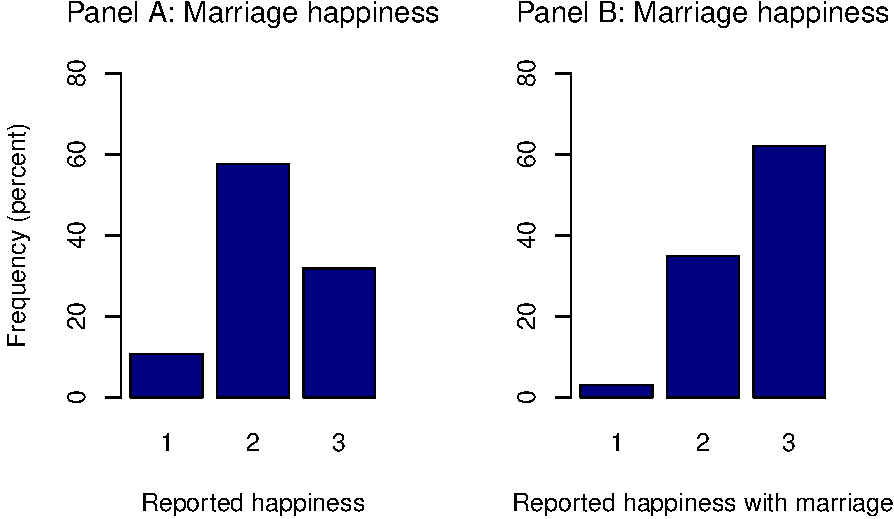
\includegraphics{Final_Project_P-P_analysis_Unger_files/figure-latex/unnamed-chunk-3-1.pdf}
\caption{Distribution of reported happiness and job-satisfaction}
\end{figure}

\subsection{Reported happiness in different survey
years}\label{reported-happiness-in-different-survey-years}

The GSS is conducted every or every other year between 1972 and 2014.
Due to year specific events, unintended differences in the
implementation of the survey or trends in overall happiness, there can
be non-random, year-specific differences. Figure 2 shows the average
share of the sample population who reports to be very happy across the
survey years.

\begin{figure}[htbp]
\centering
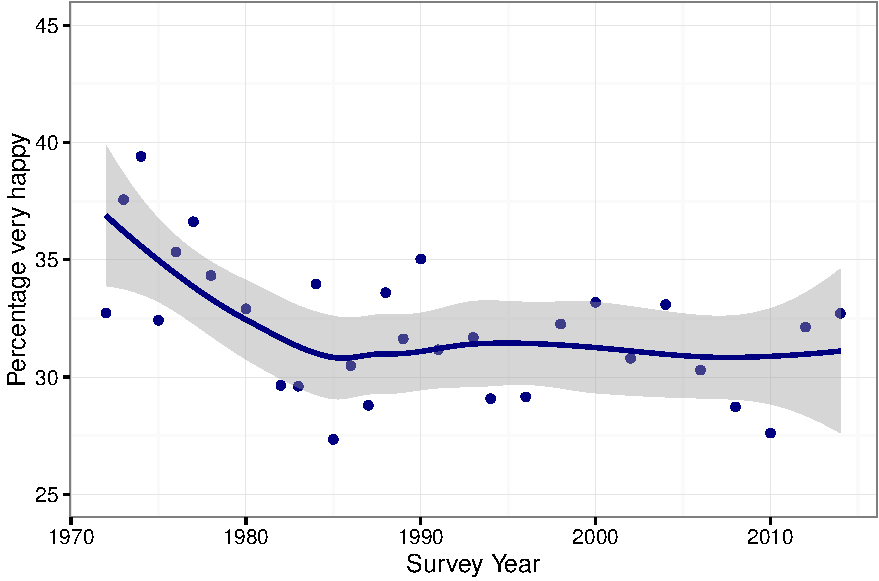
\includegraphics{Final_Project_P-P_analysis_Unger_files/figure-latex/unnamed-chunk-4-1.pdf}
\caption{Average reported happiness over survey year, 1972-2014}
\end{figure}

Figure 2 shows that there is considerable variation between years.
Furthermore, there appears to be a negative trend between 1972 and 1985.
It is not directly possible to disentangle what can be attributed to
random noise and what is caused by structural changes, however, it
signifies that it is pragmatic to control for survey year in the
regression models.

\subsection{Happiness and age}\label{happiness-and-age}

Figure 3 illustrates the relationship between reported happiness and age
for college educated men and women. In the GSS there is no apparent
structural relationship between the share of respondents who report
being very happy and age. Furthermore, college educated women have a
slightly higher average reported happiness level relative to men (38\%
vs.~34\%).

\begin{figure}[htbp]
\centering
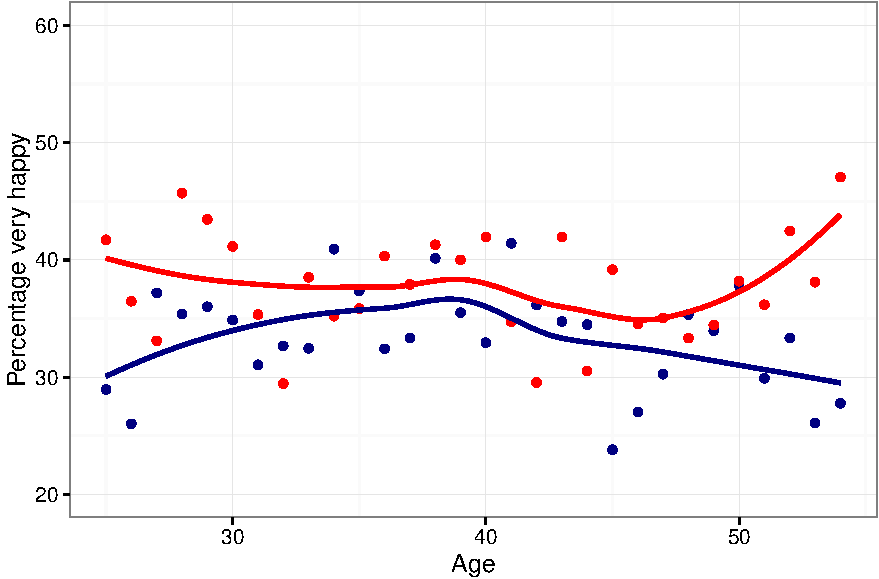
\includegraphics{Final_Project_P-P_analysis_Unger_files/figure-latex/unnamed-chunk-5-1.pdf}
\caption{Happiness and age (college educated men and women)}
\end{figure}

\subsection{Respondent's income and reported
happiness}\label{respondents-income-and-reported-happiness}

Figure 4 shows the distribution of respondents' annual income in 2009
USD for college educated men and women. We can deduce that more men than
women report high income. Furthermore, it shows that more women than men
report no income at all, either due to unemployment or because they
voluntarily keep house.

\begin{figure}[htbp]
\centering
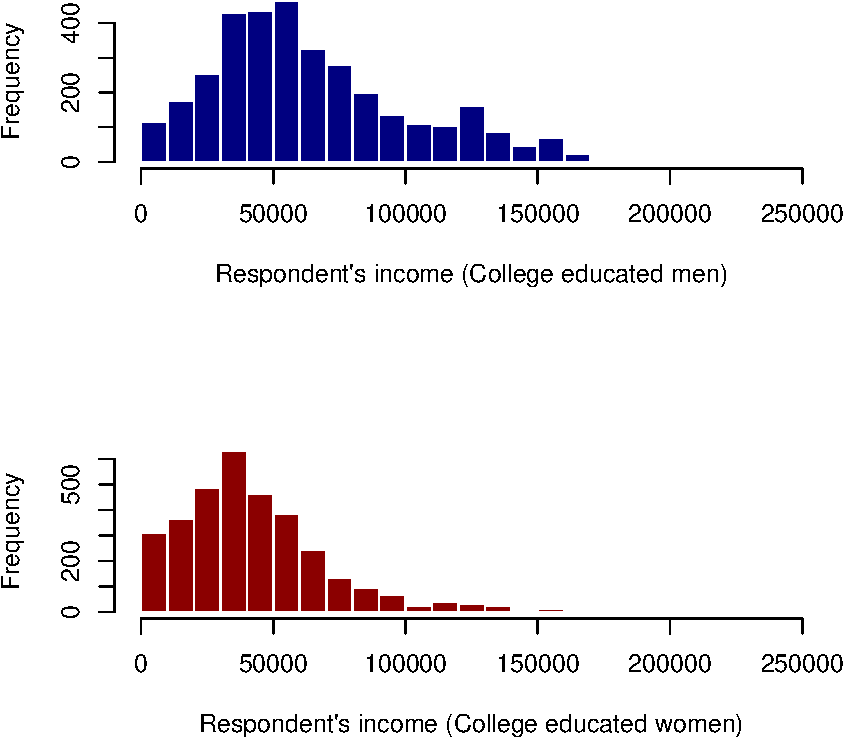
\includegraphics{Final_Project_P-P_analysis_Unger_files/figure-latex/unnamed-chunk-6-1.pdf}
\caption{Distribution of income}
\end{figure}

Figure 5 shows the correlation between respondents income and the
propensity to report high happiness for college educated women and men.
For both genders there are a positive trend, which aligns with the
majority of reserach on income and happiness {[}INSERT A REF{]}. A large
share of women with very low or no income, however, also report high
happiness. This reflects that married women who keeps house tend to
report high happiness, which we will return to in the analysis.

\begin{figure}[htbp]
\centering
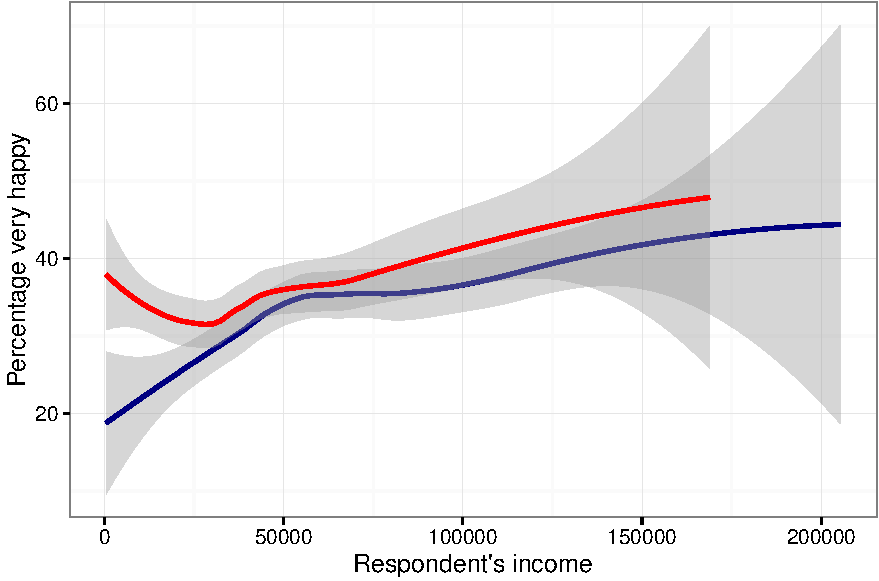
\includegraphics{Final_Project_P-P_analysis_Unger_files/figure-latex/unnamed-chunk-7-1.pdf}
\caption{Happiness and respondent's income (college educated men and
women)}
\end{figure}

\subsection{Work, household constallations and
gender}\label{work-household-constallations-and-gender}

In this section we explore how reported happiness depend on labour
market affiliation and family constellation for women and men, and
discern gender differences. All figures are restricted to college
educated women and men.

Figure 6 shows how reported happiness depends on labour-market
affiliation for men (blue) and women (red) with a college degree. It
shows that men are substantially more likely to report being very happy
when in full-time employment relative to part-time employment, which is
not the case for women. Furthermore, both men and women report high
happiness levels when keeping house. Note, however, that there are only
35 college educated men in the full sample who keep house, whereas there
are 650 women. When looking at all men, the average share who reports
being very happy while keeping house is only 24 \%.

\begin{figure}[htbp]
\centering
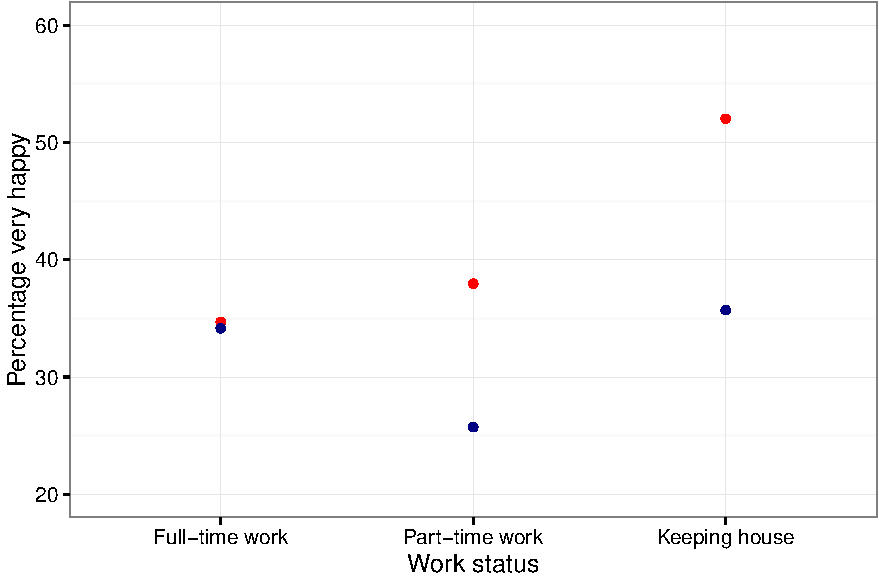
\includegraphics{Final_Project_P-P_analysis_Unger_files/figure-latex/unnamed-chunk-8-1.pdf}
\caption{Happiness and labour-market affiliation (college educated men
and women)}
\end{figure}

An important measure in our analysis is whether individuals have a
high-income. Figure 7 shows the share of college educated men and women
who report being very happy depending on whether they earn more than the
25th (panel A) or 50th (panel B) income percentile of college educated
men in their age cohort. The graph suggests that women have the same
propensity to be very happe regardless of whether they are high earners
or not, whereas the difference is substantial for men. The difference
for men is even more pronounced when the threshold is set at the 50th
percentile.

\begin{figure}[htbp]
\centering
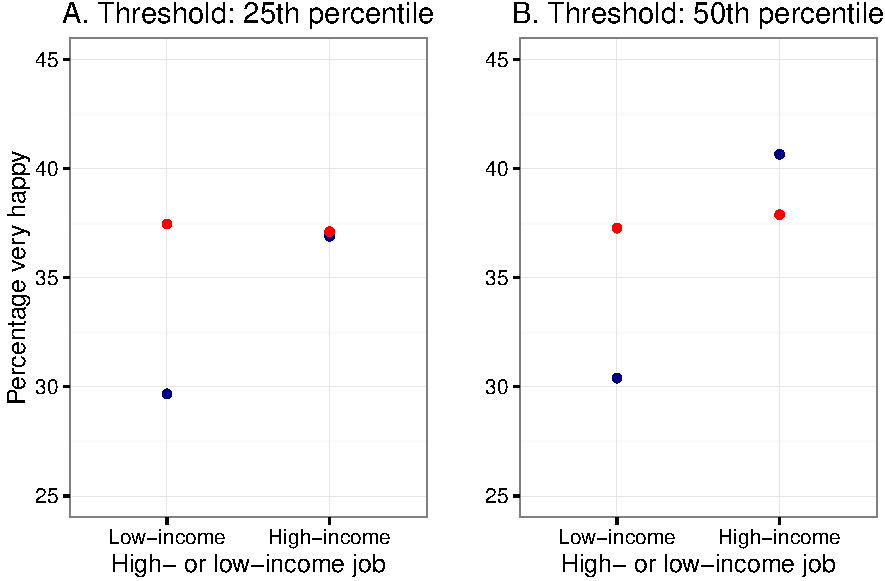
\includegraphics{Final_Project_P-P_analysis_Unger_files/figure-latex/unnamed-chunk-9-1.pdf}
\caption{Happiness and income level}
\end{figure}

\begin{table}[]
\centering
\caption{Gender, income (p50) and spouse work status (row percentages)}
\label{my-label}
\begin{tabular}{llllll}
\hline
       &             & Full-time & Part-time & Keeping house & n    \\ \hline
Female & High-income & 92.45     & 4.15      & 3.4           & 265  \\
       & Low-income  & 95.62     & 0.99      & 3.39          & 1713 \\
Male   & High-income & 42.28     & 33.56     & 24.16         & 745  \\
       & Low-income  & 54.86     & 25.06     & 20.08         & 1285 \\ \hline
\end{tabular}
\end{table}

\begin{table}[]
\centering
\caption{Gender, income (p25) and spouse work status (row percentages)}
\label{my-label}
\begin{tabular}{llllll}
\hline
       &             & Full-time & Part-time & Keeping house & n    \\ \hline
Female & High-income & 94.1      & 3.04      & 2.86          & 559  \\
       & Low-income  & 95.63     & 0.78      & 3.59          & 1419 \\
Male   & High-income & 47.71     & 28.98     & 23.31         & 1201 \\
       & Low-income  & 53.92     & 27.02     & 19.06         & 829  \\ \hline
\end{tabular}
\end{table}

\section{Analysis}\label{analysis}

\textbf{I think we should start our analysis section here.} But we of
course needs a real analysis introduction.

\subsection{Marriage / family constellation, income and
happiness}\label{marriage-family-constellation-income-and-happiness}

\textbf{}

Figure 7 differentiates between the four possible combinations of having
a family (married and children) and having a high- or low-income job
(defined as earning more than the 25th income percentile of college
educated men in the respondent's cohort). Both college educated men and
women report substantially higher happiness levels when having a family.
When not having a family, higher income improves life satisfaction for
both genders although the increase is larger for men. Gender differences
become more pronounced when people have a family. With a family, women
are happier when they are not in a high-income job, whereas the opposite
is true for men.

These descriptive results suggest that on average married couples with
kids are best-off when following a male bread-winner model, which
conflicts with more progressive gender norms. Note, however, that the
results could be driven by omitted factors such as assymetric total
family income or age across the family constellations which also could
affect subjective well-being. In our final analysis we seek to identify
the factors that are driving these results.

\textbf{Figure: Happiness and marriage/income constellation.}

\begin{figure}[htbp]
\centering
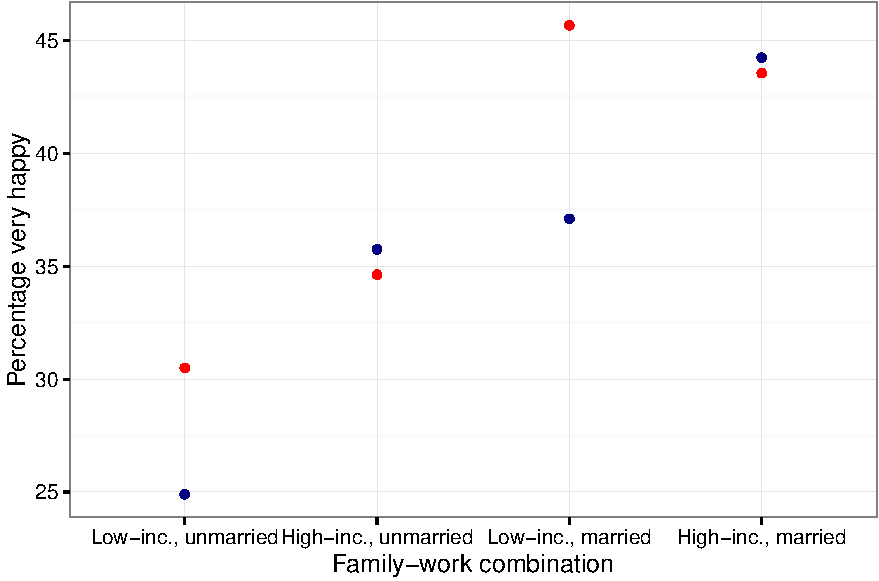
\includegraphics{Final_Project_P-P_analysis_Unger_files/figure-latex/unnamed-chunk-10-1.pdf}
\caption{Happiness and marriage constellation (college educated
subsample)}
\end{figure}

\subsection{\texorpdfstring{Interaction effects of marriage and job
income for working men and women
\emph{}.}{Interaction effects of marriage and job income for working men and women .}}\label{interaction-effects-of-marriage-and-job-income-for-working-men-and-women-.}

The correlations shown in Figure X-Y are influenced by omitted factors.
To control for some of the confounding factors that are observable, we
replicate a linear probability model by Bertrand (2013) and estimate the
effect of marriage and the interaction effect of marriage and having a
high-paid job (career) on the binary variable of being very happy. While
Bertrand (2013) limits her analysis to college-educated women who are
working, we also compare these findings to college educated men. The
model controls for age, age-squared, the survey year, race and decade of
birth.

Figure 9 shows the effect of marriage on the probability of being very
happy for college educated men and women depending on job income. First,
the effect of marriage is positive and significantly different from zero
regardless of respondents' income level. The left panel shows that the
effect of marriage on reported happiness is stronger for women who do
not have a high-income job compared to women who do, as the interaction
term between marriage and high job income is -0.07. Although this
difference only is significant at the 10\% level, job income seem to be
much more important for the happiness of women compared to men, where
having a high-paying job or not hardly influences the effect of marriage
on happiness.

\textbf{Table 1: Happiness, marriage and high-income}

\begin{table}[!htbp] \centering 
  \caption{Happiness, marriage and income for college educated men and women} 
  \label{} 
\begin{tabular}{@{\extracolsep{5pt}}lcccc} 
\\[-1.8ex]\hline 
\hline \\[-1.8ex] 
 & \multicolumn{4}{c}{\textit{Dependent variable:}} \\ 
\cline{2-5} 
\\[-1.8ex] & \multicolumn{4}{c}{Very happy} \\ 
 & Women & Men & Women & Men \\ 
\\[-1.8ex] & (1) & (2) & (3) & (4)\\ 
\hline \\[-1.8ex] 
 High-income & 7.79$^{**}$ & 8.00$^{**}$ & 6.92$^{*}$ & 8.10$^{***}$ \\ 
  & (3.17) & (3.61) & (3.53) & (3.11) \\ 
  & & & & \\ 
 Married & 18.98$^{***}$ & 21.00$^{***}$ & 21.61$^{***}$ & 17.46$^{***}$ \\ 
  & (2.09) & (1.84) & (1.79) & (2.03) \\ 
  & & & & \\ 
 High-income*Married & 0.02 & $-$9.94$^{**}$ & $-$9.96$^{**}$ & 0.18 \\ 
  & (3.84) & (4.84) & (4.83) & (3.81) \\ 
  & & & & \\ 
 Constant & 21.55 & 105.73$^{***}$ & 24.84$^{***}$ & 20.22$^{***}$ \\ 
  & (26.01) & (25.99) & (1.36) & (1.55) \\ 
  & & & & \\ 
\hline \\[-1.8ex] 
Age & Yes & Yes & No & No \\ 
Age-squared & Yes & Yes & No & No \\ 
Year & Yes & Yes & No & No \\ 
Race & Yes & Yes & No & No \\ 
Cohort & Yes & Yes & No & No \\ 
\hline \\[-1.8ex] 
Observations & 3,119 & 3,309 & 3,309 & 3,119 \\ 
Adjusted R$^{2}$ & 0.05 & 0.05 & 0.04 & 0.04 \\ 
\hline 
\hline \\[-1.8ex] 
\textit{Note:}  & \multicolumn{4}{r}{$^{*}$p$<$0.1; $^{**}$p$<$0.05; $^{***}$p$<$0.01} \\ 
 & \multicolumn{4}{r}{Models are restricted to college educated men and women} \\ 
\end{tabular} 
\end{table}

\emph{NOTE: Table1: There is a problem with the omit.labels function.}

\textbf{Figure: Interaction between marriage and high-income}

\begin{figure}[htbp]
\centering
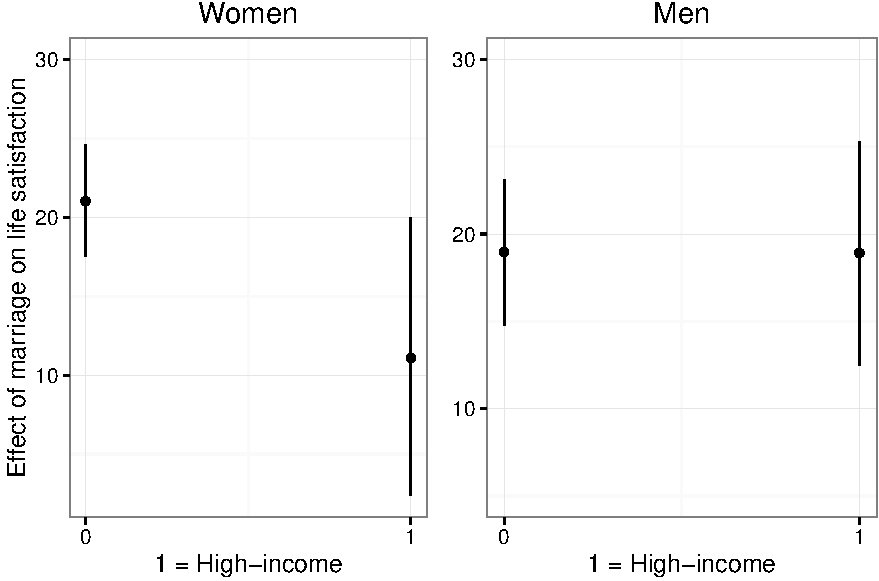
\includegraphics{Final_Project_P-P_analysis_Unger_files/figure-latex/unnamed-chunk-12-1.pdf}
\caption{Interaction effects of marriage and job income on life
satisfaction}
\end{figure}

\subsection{Double-click on married respondent's: How does high-income
differ between
genders?}\label{double-click-on-married-respondents-how-does-high-income-differ-between-genders}

\textbf{Table 2: Double-click on married individuals}

\begin{table}[!htbp] \centering 
  \caption{Happiness and work-status for married, college educated women and men} 
  \label{} 
\begin{tabular}{@{\extracolsep{5pt}}lcccc} 
\\[-1.8ex]\hline 
\hline \\[-1.8ex] 
 & \multicolumn{4}{c}{\textit{Dependent variable:}} \\ 
\cline{2-5} 
\\[-1.8ex] & \multicolumn{4}{c}{Very happy} \\ 
 & Women & Men & Women & Men \\ 
\\[-1.8ex] & (1) & (2) & (3) & (4)\\ 
\hline \\[-1.8ex] 
 High-income & $-$0.55 & 8.34$^{***}$ & 2.19 & 8.37$^{***}$ \\ 
  & (3.51) & (2.34) & (3.86) & (2.79) \\ 
  & & & & \\ 
 Keeping house & 14.46$^{***}$ & $-$4.52 & 7.27$^{*}$ & $-$1.91 \\ 
  & (2.91) & (14.20) & (3.75) & (14.65) \\ 
  & & & & \\ 
 Child & $-$5.40$^{*}$ & $-$4.65$^{*}$ & $-$2.16 & $-$2.41 \\ 
  & (2.76) & (2.76) & (3.01) & (3.04) \\ 
  & & & & \\ 
 Constant & 47.32$^{***}$ & 41.34$^{***}$ & 171.03$^{***}$ & 47.75 \\ 
  & (2.47) & (2.56) & (37.68) & (37.45) \\ 
  & & & & \\ 
\hline \\[-1.8ex] 
Partner's income & No & No & No & No \\ 
Age & No & No & No & No \\ 
Age-squared & No & No & No & No \\ 
Year & No & No & No & No \\ 
Race & No & No & No & No \\ 
Cohort & No & No & No & No \\ 
\hline \\[-1.8ex] 
Observations & 1,881 & 1,928 & 1,881 & 1,928 \\ 
Adjusted R$^{2}$ & 0.01 & 0.01 & 0.03 & 0.02 \\ 
\hline 
\hline \\[-1.8ex] 
\textit{Note:}  & \multicolumn{4}{r}{$^{*}$p$<$0.1; $^{**}$p$<$0.05; $^{***}$p$<$0.01} \\ 
 & \multicolumn{4}{r}{Models include married, college educated men and women} \\ 
\end{tabular} 
\end{table}

\{\tiny{Models include married, college educated men and women}\}

\textbf{Table 2: The omit.label function is still bugging!!!!!!!!}

\subsection{Effect on happiness of young
children}\label{effect-on-happiness-of-young-children}

\textbf{Table 3: Happiness and young children}

\begin{table}[!htbp] \centering 
  \caption{Happiness and young children, college educated women and men with a family} 
  \label{} 
\begin{tabular}{@{\extracolsep{5pt}}lcccccc} 
\\[-1.8ex]\hline 
\hline \\[-1.8ex] 
 & \multicolumn{6}{c}{\textit{Dependent variable:}} \\ 
\cline{2-7} 
\\[-1.8ex] & \multicolumn{6}{c}{Very happy} \\ 
 & Women & Men & Women & Men & Women & Men \\ 
\\[-1.8ex] & (1) & (2) & (3) & (4) & (5) & (6)\\ 
\hline \\[-1.8ex] 
 High-income & 1.39 & 7.11$^{***}$ & 6.33 & 6.04$^{*}$ & 9.40$^{*}$ & 5.69 \\ 
  & (4.18) & (2.60) & (4.64) & (3.15) & (5.35) & (3.58) \\ 
  & & & & & & \\ 
 Keeping house & 14.40$^{***}$ & $-$3.80 & 6.61 & $-$3.07 & 5.29 &  \\ 
  & (3.06) & (16.36) & (4.12) & (16.62) & (4.86) &  \\ 
  & & & & & & \\ 
 Young child &  &  &  &  & 4.82 & 1.90 \\ 
  &  &  &  &  & (4.44) & (3.82) \\ 
  & & & & & & \\ 
 Keeping House*Young child &  &  &  &  & 1.89 &  \\ 
  &  &  &  &  & (6.49) &  \\ 
  & & & & & & \\ 
 High-income*Young child &  &  &  &  & $-$11.13 & 1.51 \\ 
  &  &  &  &  & (9.63) & (5.95) \\ 
  & & & & & & \\ 
 Constant & 41.72$^{***}$ & 37.14$^{***}$ & 119.85$^{**}$ & 34.88 & 99.94$^{**}$ & 27.75 \\ 
  & (1.62) & (1.57) & (46.79) & (46.47) & (49.15) & (47.55) \\ 
  & & & & & & \\ 
\hline \\[-1.8ex] 
Partner's income & No & No & No & No & No & No \\ 
Age & No & No & No & No & No & No \\ 
Age-squared & No & No & No & No & No & No \\ 
Year & No & No & No & No & No & No \\ 
Race & No & No & No & No & No & No \\ 
Cohort & No & No & No & No & No & No \\ 
\hline \\[-1.8ex] 
Observations & 1,448 & 1,529 & 1,448 & 1,529 & 1,448 & 1,529 \\ 
Adjusted R$^{2}$ & 0.01 & 0.004 & 0.02 & 0.02 & 0.02 & 0.02 \\ 
\hline 
\hline \\[-1.8ex] 
\textit{Note:}  & \multicolumn{6}{r}{$^{*}$p$<$0.1; $^{**}$p$<$0.05; $^{***}$p$<$0.01} \\ 
 & \multicolumn{6}{r}{Models are restricted to married + child, college educated men and women} \\ 
\end{tabular} 
\end{table}

\textbf{Needs to be populated}

There story remains relatively weak. We don't have a significant
negative interaction term, partly because we have less than 50
individuals that have both career1 and a young child.

Nonetheless, we can argue that at least it seems to be the career
individuals with a young child that reports low life hapiness.

Do we have a problem of maternity leave? I guess they are excluded as
they wont earn much.

\subsection{Satisfaction with marriage and family
constellation.}\label{satisfaction-with-marriage-and-family-constellation.}

\textbf{Table 4: Marriage happiness and spouse working conditions}

\begin{table}[!htbp] \centering 
  \caption{Marriage happiness and spouse's work-status} 
  \label{} 
\begin{tabular}{@{\extracolsep{5pt}}lcccccc} 
\\[-1.8ex]\hline 
\hline \\[-1.8ex] 
 & \multicolumn{6}{c}{\textit{Dependent variable:}} \\ 
\cline{2-7} 
\\[-1.8ex] & \multicolumn{6}{c}{Very happy (marriage)} \\ 
 & Women & Men & Women & Men & Women & Men \\ 
\\[-1.8ex] & (1) & (2) & (3) & (4) & (5) & (6)\\ 
\hline \\[-1.8ex] 
 Spouse FT & 6.44 & $-$0.97 & 14.03 & $-$8.42$^{*}$ & 15.87 & $-$10.12$^{*}$ \\ 
  & (5.26) & (2.89) & (11.93) & (4.85) & (12.69) & (5.35) \\ 
  & & & & & & \\ 
 Spouse Home &  & 2.17 &  & 4.03 &  & 4.99 \\ 
  &  & (3.16) &  & (4.95) &  & (5.23) \\ 
  & & & & & & \\ 
 Children & $-$8.09$^{***}$ & $-$1.67 & 3.31 & $-$3.21 &  &  \\ 
  & (2.93) & (3.09) & (7.97) & (5.46) &  &  \\ 
  & & & & & & \\ 
 Constant & 150.03$^{***}$ & 154.04$^{***}$ & 145.45 & 231.51$^{**}$ & 163.19 & 244.38$^{**}$ \\ 
  & (38.23) & (37.79) & (133.90) & (93.70) & (166.64) & (110.32) \\ 
  & & & & & & \\ 
\hline \\[-1.8ex] 
Family income & Yes & Yes & Yes & Yes & Yes & Yes \\ 
Age & Yes & Yes & Yes & Yes & Yes & Yes \\ 
Age-squared & Yes & Yes & Yes & Yes & Yes & Yes \\ 
Year & Yes & Yes & Yes & Yes & Yes & Yes \\ 
Race & Yes & Yes & Yes & Yes & Yes & Yes \\ 
Cohort & Yes & Yes & Yes & Yes & Yes & Yes \\ 
\hline \\[-1.8ex] 
Observations & 1,746 & 1,830 & 222 & 646 & 156 & 535 \\ 
Adjusted R$^{2}$ & 0.03 & 0.02 & 0.04 & 0.04 & 0.06 & 0.05 \\ 
\hline 
\hline \\[-1.8ex] 
\textit{Note:}  & \multicolumn{6}{r}{$^{*}$p$<$0.1; $^{**}$p$<$0.05; $^{***}$p$<$0.01} \\ 
 & \multicolumn{6}{r}{Models are restricted to married, college educated men and women} \\ 
\end{tabular} 
\end{table}

\textbf{We need to shine up the table and indicate (3) and (4) is for
career1 == 1}

Text: The story needs to be pushed here again. Problem is that people
presumably choose the career constellations they believe they will be
happy in.

We should probably add the contingency tables here.

Question to be answered: Do we also report life happiness and family
constellation? Problem is that career women actually prefer their
husband to not work full-time :/ It could work as a story, but does
hardly align with the lower marriage happiness.

Another meth. problem: A full-time job is not necessarily intensive. 40
hours a week is not unmanageble. Problem is that we don't have a better
variable.

\subsection{Cohorts and norms}\label{cohorts-and-norms}

\textbf{Populate with text.}

\textbf{Figure: Cohortian differences}

\begin{figure}[htbp]
\centering
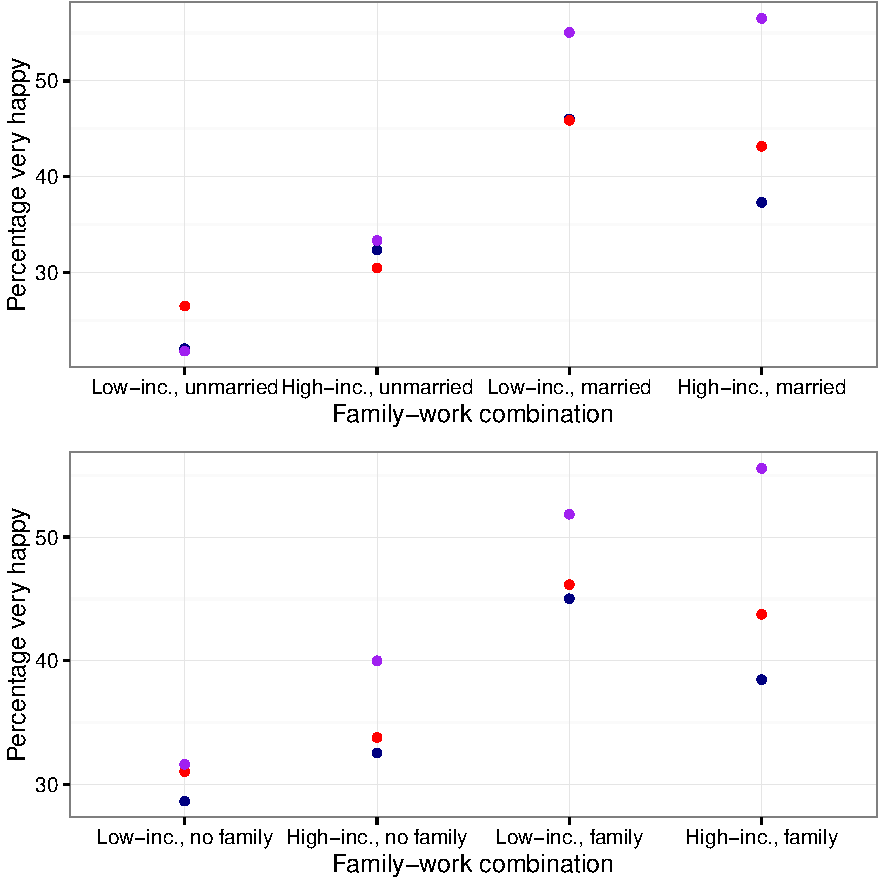
\includegraphics{Final_Project_P-P_analysis_Unger_files/figure-latex/unnamed-chunk-16-1.pdf}
\caption{Happiness and family constellation (college educated women)}
\end{figure}

\section{Discussion}\label{discussion}

\section{Conclusion}\label{conclusion}

The preliminary analyses indicate that some variation in reported
happiness is associated with job-affiliation and gender. Further, our
descriptive results suggest that determinants for happiness, such as
having a family or high job-income, differ in magnitude and direction
between genders. This supports our initial assumption of differences in
reconcilability of a career pursuit and a happy life. However, it
remains a challenge to construct models which can attenuate problems of
confounding factors. For the final project we intend to investigate in
more detail how the intensity of work influences happiness and whether
there is a trade-off between job satisfaction and overall hapiness.

\section{Software and packages used for the
analysis}\label{software-and-packages-used-for-the-analysis}

The analysis is done in R (R Core Team 2015b) with the use of the
following packages: ``ggplot2'' (Wickham and Chang 2015), ``repmis''
(Gandrud 2016), ``plyr'' (Wickham 2015), ``dplyr'' (Wickham and Francois
2015), ``MASS'' (Ripley 2015), ``Hmisc'' (Harrell 2016), ``interplot''
(Solt and Hu 2016), ``gridExtra'' (Auguie 2016), ``car'' (Fox and
Weisberg 2016), ``foreign'' (R Core Team 2015a), ``gmodels'' (Warnes et
al. 2015), ``quantmod'' (Ryan 2015) and ``reshape'' (Wickham 2014).

\section*{References}\label{references}
\addcontentsline{toc}{section}{References}

\hypertarget{refs}{}
\hypertarget{ref-R-gridExtra}{}
Auguie, Baptiste. 2016. \emph{GridExtra: Miscellaneous Functions for
``Grid'' Graphics}. \url{https://CRAN.R-project.org/package=gridExtra}.

\hypertarget{ref-bertrand2013}{}
Bertrand, Marianne. 2013. ``Career, Family, and the Well-Being of
College-Educated Women.'' \emph{The American Economic Review} 103 (3).
American Economic Association: 244--50.

\hypertarget{ref-R-car}{}
Fox, John, and Sanford Weisberg. 2016. \emph{Car: Companion to Applied
Regression}. \url{https://CRAN.R-project.org/package=car}.

\hypertarget{ref-R-repmis}{}
Gandrud, Christopher. 2016. \emph{Repmis: Miscellaneous Tools for
Reproducible Research}. \url{https://CRAN.R-project.org/package=repmis}.

\hypertarget{ref-R-Hmisc}{}
Harrell, Frank E, Jr. 2016. \emph{Hmisc: Harrell Miscellaneous}.
\url{https://CRAN.R-project.org/package=Hmisc}.

\hypertarget{ref-R-foreign}{}
R Core Team. 2015a. \emph{Foreign: Read Data Stored by Minitab, S, SAS,
SPSS, Stata, Systat, Weka, DBase, .}
\url{https://CRAN.R-project.org/package=foreign}.

\hypertarget{ref-CiteR}{}
---------. 2015b. \emph{R: A Language and Environment for Statistical
Computing}. Vienna, Austria: R Foundation for Statistical Computing.
\url{https://www.R-project.org/}.

\hypertarget{ref-R-MASS}{}
Ripley, Brian. 2015. \emph{MASS: Support Functions and Datasets for
Venables and Ripley's MASS}.
\url{https://CRAN.R-project.org/package=MASS}.

\hypertarget{ref-R-quantmod}{}
Ryan, Jeffrey A. 2015. \emph{Quantmod: Quantitative Financial Modelling
Framework}. \url{https://CRAN.R-project.org/package=quantmod}.

\hypertarget{ref-R-interplot}{}
Solt, Frederick, and Yue Hu. 2016. \emph{Interplot: Plot the Effects of
Variables in Interaction Terms}.
\url{https://CRAN.R-project.org/package=interplot}.

\hypertarget{ref-R-gmodels}{}
Warnes, Gregory R., Ben Bolker, Thomas Lumley, Randall C Johnson.
Contributions from Randall C. Johnson are Copyright SAIC-Frederick, Inc.
Funded by the Intramural Research Program, of the NIH, National Cancer
Institute, and Center for Cancer Research under NCI Contract
NO1-CO-12400. 2015. \emph{Gmodels: Various R Programming Tools for Model
Fitting}. \url{https://CRAN.R-project.org/package=gmodels}.

\hypertarget{ref-R-reshape}{}
Wickham, Hadley. 2014. \emph{Reshape: Flexibly Reshape Data.}
\url{https://CRAN.R-project.org/package=reshape}.

\hypertarget{ref-R-plyr}{}
---------. 2015. \emph{Plyr: Tools for Splitting, Applying and Combining
Data}. \url{https://CRAN.R-project.org/package=plyr}.

\hypertarget{ref-R-ggplot2}{}
Wickham, Hadley, and Winston Chang. 2015. \emph{Ggplot2: An
Implementation of the Grammar of Graphics}.
\url{https://CRAN.R-project.org/package=ggplot2}.

\hypertarget{ref-R-dplyr}{}
Wickham, Hadley, and Romain Francois. 2015. \emph{Dplyr: A Grammar of
Data Manipulation}. \url{https://CRAN.R-project.org/package=dplyr}.

\end{document}
